% Latex template: mahmoud.s.fahmy@students.kasralainy.edu.eg
% For more details: https://www.sharelatex.com/learn/Beamer

\documentclass{beamer}					% Document class

\setbeamertemplate{footline}[text line]{%
  \parbox{\linewidth}{\vspace*{-8pt}Feature Selection\hfill\insertshortauthor\hfill\insertpagenumber}}
\setbeamertemplate{navigation symbols}{}

\usepackage[english]{babel}				% Set language
\usepackage[utf8x]{inputenc}			% Set encoding

\mode<presentation>						% Set options
{
  \usetheme{default}					% Set theme
  \usecolortheme{default} 				% Set colors
  \usefonttheme{default}  				% Set font theme
  \setbeamertemplate{caption}[numbered]	% Set caption to be numbered
}

% Uncomment this to have the outline at the beginning of each section highlighted.
%\AtBeginSection[]
%{
%  \begin{frame}{Outline}
%    \tableofcontents[currentsection]
%  \end{frame}
%}

\usepackage{graphicx}					% For including figures
\usepackage{booktabs}					% For table rules
\usepackage{hyperref}					% For cross-referencing
\usepackage{bm}
\usepackage{algorithm,algorithmic}

\title{Feature Selection}	% Presentation title
\author{Clayton W. Seitz}								% Presentation author
\date{\today}									% Today's date	

\begin{document}

% Title page
% This page includes the informations defined earlier including title, author/s, affiliation/s and the date
\begin{frame}
  \titlepage
\end{frame}

% The following is the most frequently used slide types in beamer
% The slide structure is as follows:
%
%\begin{frame}{<slide-title>}
%	<content>
%\end{frame}

\begin{frame}{Feature Selection and Extraction}

\begin{center}
\begin{figure}
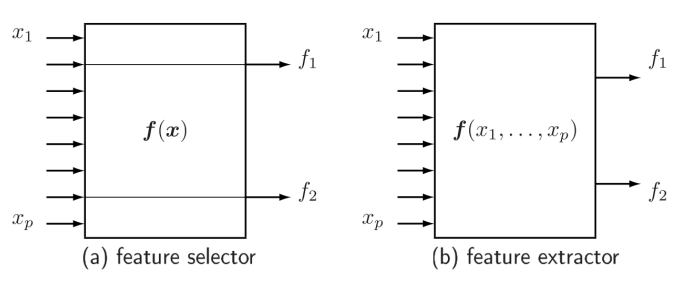
\includegraphics[width=1.0\textwidth]{features.png}
\end{figure}
\end{center}
\end{frame}

\begin{frame}{Feature Selection}

What is it?\\
\vspace{0.2in}
A special type of dimensionality reduction where we select a subset of features, in contrast with feature extraction like in PCA, VAE\\
\vspace{0.2in}
Why do we do it? \\
\vspace{0.2in}
\begin{itemize}
\item Quality of the input data is just as important as the algorithm you choose
\item The volume of a feature space grows exponentially in the number of dimensions $n$
\item But we often have a small number of samples $p<<n$
\end{itemize}

\end{frame}

\begin{frame}{Probabilistic Distance Measures}
\vspace{0.2in}
How do we define a notion of distance for probability distributions?
\begin{center}
\begin{figure}
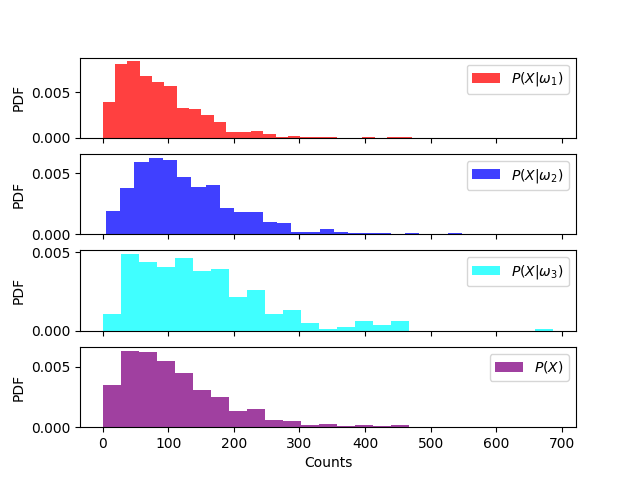
\includegraphics[width=0.9\textwidth]{hists.png}
\end{figure}
\end{center}
\end{frame}

\begin{frame}{Symmetric Kullbeck-Leibler (KL) Divergence}

The standard definition of KL-Divergence is 

The form that has been used in feature selection for classification tasks reads

\begin{equation*}
S = D_{KL}(P||Q) + D_{KL}(Q||P)
\end{equation*}

The major drawback of univariate methods is that we do not consider contextual changes 

\end{frame}

\begin{frame}{Result}
\begin{center}
\begin{figure}
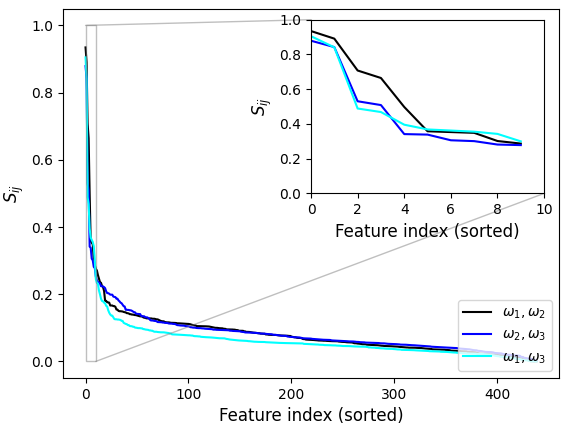
\includegraphics[width=0.9\textwidth]{kld.png}
\end{figure}
\end{center}
%$(\omega_{1},\omega_{2},\omega_{3}) = (ctrl,t1d,aabp)$
\end{frame}

\section{References}

% Adding the option 'allowframebreaks' allows the contents of the slide to be expanded in more than one slide.
\begin{frame}[allowframebreaks]{References}
	\tiny\bibliography{references}
	\bibliographystyle{apalike}
\end{frame}

\end{document}